% !TEX root = ../Thesis.tex
\chapter{Background}
\label{ch:background}

\begingroup
\setaftersecskip{6pt}
\setlength{\emergencystretch}{2em}
This chapter describes the technical background of the VR museum. It first explains multimedia retrieval, semantic search and vector representations. It then presents CLIP and shows how the CLIP principle can be applied to 3D models. Finally, it describes the vitrivr-engine, which provides the search backend for this thesis.


\section{Multimedia Retrieval}
\label{sec:background-multimedia-retrieval}

Multimedia retrieval means searching collections of images, videos, audio files or other media types. The search can use both existing metadata and the content of a medium. It can use features that can be calculated, such as color, texture, shape and motion \citep{flickner1995qbic}. vitrivr applies this principle to a modular retrieval stack with several query types \citep{rossetto2016vitrivr}.

In vitrivr-engine, a \emph{descriptor} extracts a feature from a media item. This feature can be a single value, such as an average color value or a vector created by a neural network. A media item can have several such features \citep{gasser2020cottontail,gasser2024engine}. Vectors can generally capture more complex features of a medium.

\section{Semantic Search and Vector Representations}
\label{sec:background-vector-representations}

A feature can be represented numerically as a feature vector. In the vector space model, a media object is shown as a point in a space with many dimensions \citep{gasser2020cottontail}. A trained \emph{embedding model} creates such vector representations \citep{seyedmonir2024vectorsearch,radford2021clip}. The similarity of two items is found from the distance between their vectors. In shared image-text embeddings, images and texts with related meanings should be close to each other \citep{radford2021clip,waltenspuel2024crossmodal}.

For a search, the query is also represented as a vector. The system compares it with the stored vectors and finds the nearest neighbors \citep{seyedmonir2024vectorsearch,gasser2020cottontail}. Different distance functions can be used for this comparison. For example, Cottontail DB supports Manhattan, Euclidean and cosine distance, as well as other functions \citep{gasser2020cottontail}. The descriptor and the backend decide which function is used. The nearest vectors form a ranked list, which is usually limited to the first $k$ results. The ranking therefore describes similarity according to the feature that is used.

Figure~\ref{fig:semantic-embedding-space} shows this principle in a simple example with three dimensions. The red query \emph{Computer} is also represented as a vector. Of the stored terms, \emph{CPU} is closest in meaning, so it appears first. \emph{Web Development} is related too, but less closely, so it appears later. Real embeddings have many more than three dimensions. The figure therefore shows a simple projection, not the real feature space.

\begin{figure}[htbp]
  \centering
  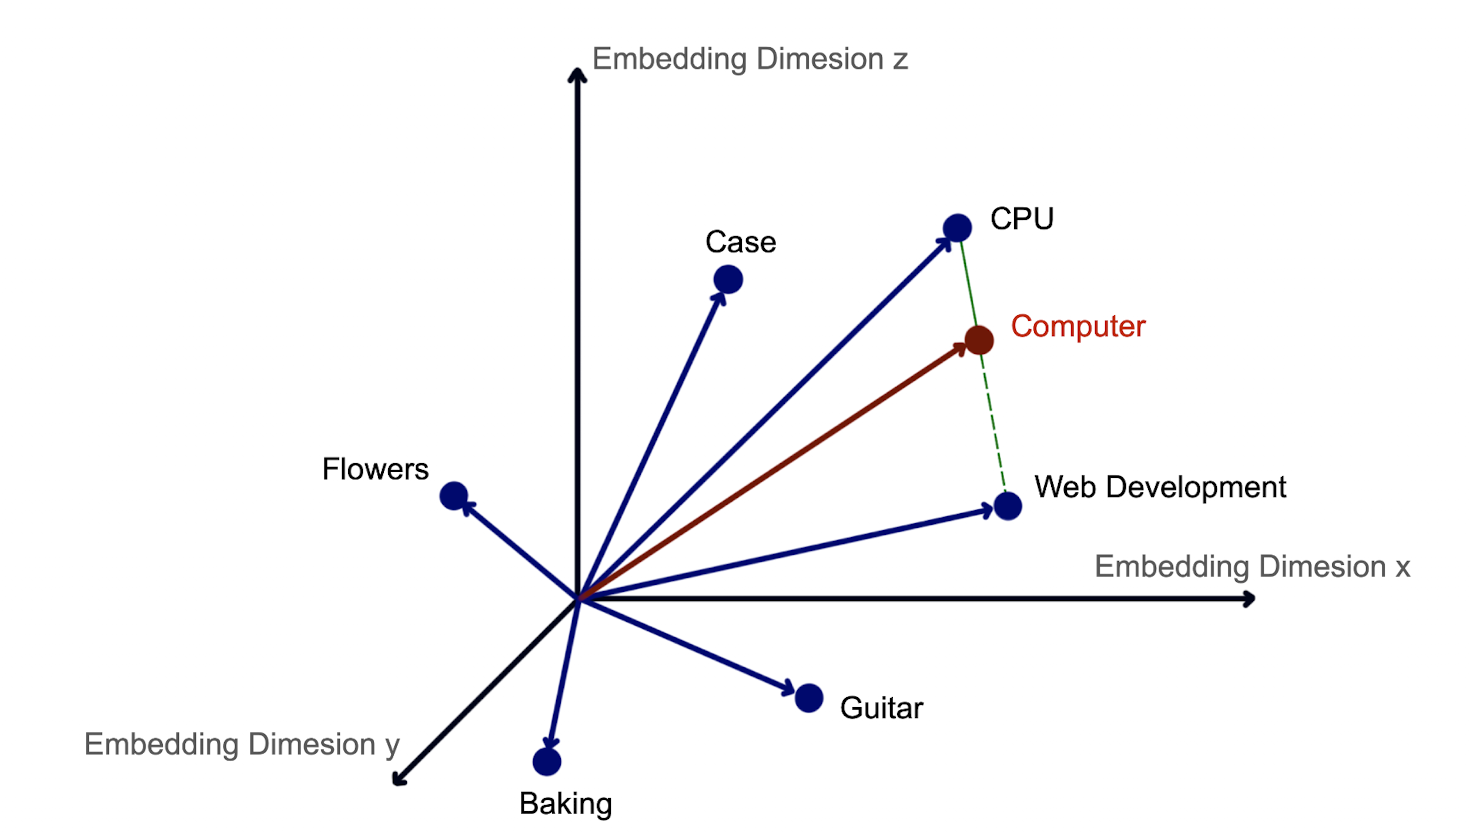
\includegraphics[width=\textwidth]{Figures/ch03-03-semantic-embedding-space.png}
  \caption[Semantic similarity in an embedding space]{
    Simple view of a query and terms with similar meanings in a three-dimensional feature space. The green marks show the order of the most similar results.
  }
  \label{fig:semantic-embedding-space}
\end{figure}

The query vector can be created from different inputs. For a text search, the description is converted into a vector. For a similarity search, the stored vector of a media object can be used as the query. If no vector is available yet, the media object is embedded in the shared feature space with the same descriptor. The query vector is then compared with the stored vectors \citep{flickner1995qbic,rossetto2016vitrivr}.

This type of example search is often called \emph{Query by Example} or \emph{More Like This}. It does not need a new text description. Instead, it uses the representation of a selected result to find its nearest neighbors. In the VR museum, this principle is the basis of the \emph{Similar} action. The vector stored with an exhibit becomes the query for the next search.

\clearpage
\section{CLIP and Multimodal Content}
\label{sec:background-clip}

For a direct comparison, text and visual media must be in the same feature space. CLIP stands for \emph{Contrastive Language--Image Pre-training}. It uses an image encoder and a text encoder. The model is trained to match related images and texts within a batch and to separate pairs that do not belong together \citep{radford2021clip}. This creates comparable representations for images and texts.

OpenCLIP is one feature descriptor used by vitrivr-engine \citep{gasser2024engine}. It provides an open-source implementation and a family of models that follow the CLIP principle \citep{cherti2023openclip}. The configuration in this thesis uses one field named \texttt{clip}, populated by a CLIP descriptor for all supported media types.

Figure~\ref{fig:visual-text-co-embedding} shows the general structure of a visual-text co-embedding in vitrivr. Video frames and text are processed through separate paths and then mapped into the same feature space. Matching videos and sentences should be close to each other, while videos that do not match should be farther away \citep{spiess2022vitrivrvr}.

\begin{figure}[htbp]
  \centering
  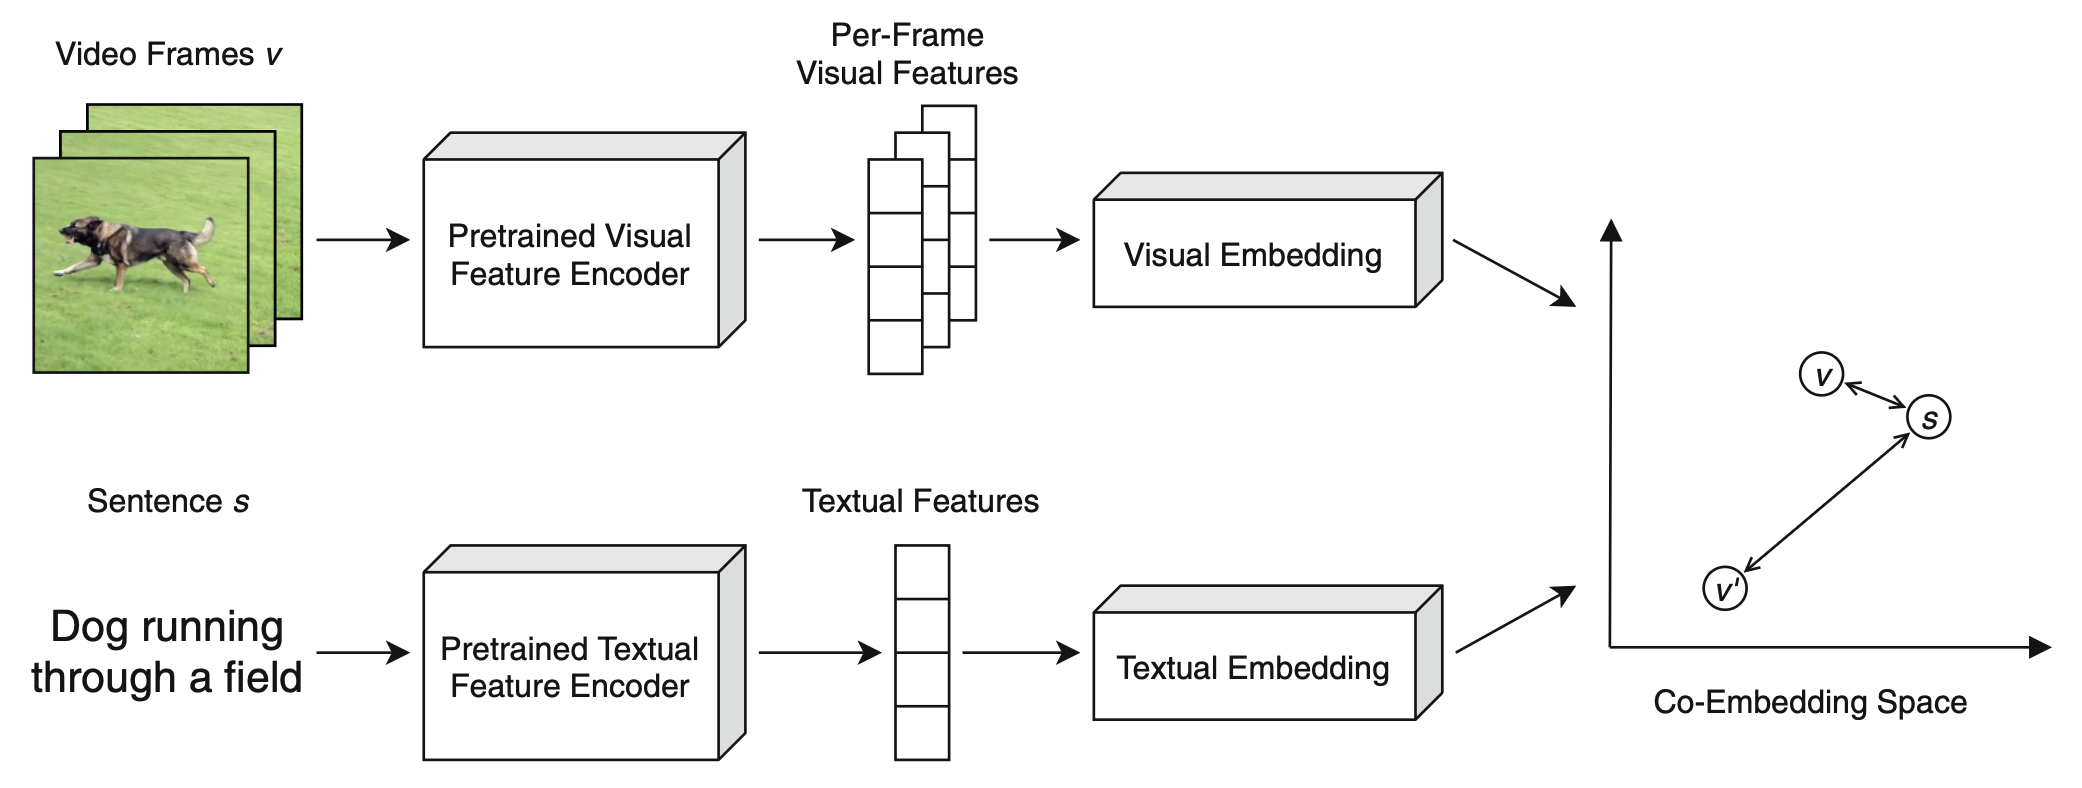
\includegraphics[width=\textwidth]{Figures/ch03-01-visual-text-co-embedding.png}
  \caption[Visual-text co-embedding in vitrivr]{
    Processing of video frames and text in separate encoder paths and mapping into a shared co-embedding space \protect\citep[Fig.~2]{spiess2022vitrivrvr}.
  }
  \label{fig:visual-text-co-embedding}
\end{figure}

After training, new images and texts can be embedded independently. This allows a text query to be compared with the visual vectors in the collection. An image vector can also be used for a similarity search.

The original CLIP model processes images and texts. Individual frames can be used for videos. MediaMix uses this method for its similarity search \citep{arnold2025mediamix}.

\clearpage
\section{Cross-Modal 3D Model Retrieval}
\label{sec:background-cross-modal-3d}

A 3D model has features such as geometry, orientation, topology and textures. Models with different file formats, numbers of vertices or texture resolutions can still look almost the same when rendered. For retrieval, this complex representation must therefore be changed into compact features that can be compared \citep{waltenspuel2024crossmodal}.

Methods for describing 3D models can be divided roughly into geometry-based and view-based approaches. Geometry-based methods use features of the spatial structure. View-based methods instead use the visible appearance. For this purpose, the model is rendered from one or more camera positions. Because of perspective and hidden parts, a single view does not always show the full shape. However, it can be processed with existing image descriptors \citep{waltenspuel2024crossmodal}.

A well-known view-based method is \emph{2D Planar View Mapping}, introduced by \citet{chen2003visualsimilarity}. It represents a 3D model through projections from several viewpoints. \citet{waltenspuel2024crossmodal} build on this idea by processing such projections with image-text embedding models.

\begin{figure}[htbp]
  \centering
  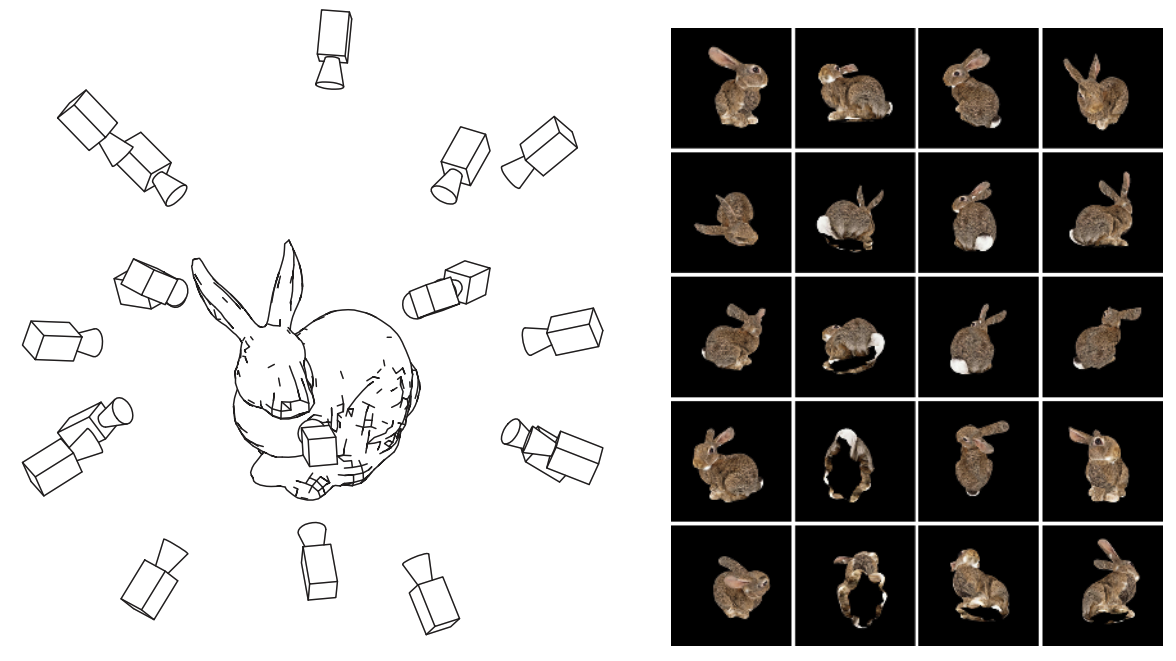
\includegraphics[width=\textwidth]{Figures/ch03-02-cross-modal-view-generation.png}
  \caption[Generation of 2D views for cross-modal 3D model retrieval]{
    Creation of two-dimensional views of a 3D model \protect\citep[Fig.~2]{waltenspuel2024crossmodal}.
  }
  \label{fig:cross-modal-rabbit}
\end{figure}

An image-text model converts each view into a vector, resulting in several vectors for one 3D model. Since some views may not show the object clearly, \citet{waltenspuel2024crossmodal} group similar vectors and combine the largest group into a single vector. This vector can then be compared with text-query vectors, enabling text-based retrieval of 3D models.

\clearpage
\section{The vitrivr Retrieval Stack}
\label{sec:background-vitrivr}

vitrivr is an open-source stack for content-based multimedia retrieval. Today, the vitrivr-engine is its main backend. It connects media preparation and feature storage with later searches. The engine has a modular design and is not tied to a specific frontend or one media type \citep{gasser2024engine}. In this thesis, the VR museum accesses the engine as a frontend.

Processing in the vitrivr-engine is split into configurable pipelines. Each pipeline is a sequence of operators with specific jobs, such as decoding a file, segmenting it, extracting a feature, searching vectors or loading additional data. The pipelines used to prepare the collection and run queries share the same data model and database connection \citep{gasser2024engine}.

During preparation, a media source is first recorded and decoded. Depending on the media type, more units can be created from it. For example, a video can be divided into time segments, while several views can be created for a 3D model. Descriptors are used to calculate the key features of each unit. The results and the relationships between them are then stored. By adjusting its configuration, the same engine can process images, videos and 3D models.


At the center of the data model are \emph{Retrievables}. A Retrievable can stand for an entire media file or for a derived part, for example a temporal segment. Fields attached to a Retrievable hold values such as feature vectors or scalar attributes. Relations can link Retrievables, for example a video file and its segments \citep{gasser2024engine}.

The vitrivr-engine presented in 2024 used Cottontail DB \citep{gasser2024engine}. MediaMix changed this setup in 2025 and uses PostgreSQL with the pgvector extension instead \citep{arnold2025mediamix,pgvector2026}. This thesis follows the MediaMix setup. Images, videos and 3D models have separate indexing pipelines, but all three write their representations to the shared \texttt{clip} field. The vitrivr Python Descriptor Server produces the CLIP vectors. PostgreSQL stores them as vectors using pgvector and makes them available for similarity search \citep{vitrivrPythonDescriptorServer2026,pgvector2026}.

In the VR museum, the backend prepares the collection and processes both text-based and vector-based queries. It then returns a ranked list of results. The frontend uses this list to choose which items fit into the virtual room, present them as exhibits, and allow users to continue exploring through new searches.

\endgroup
